\section{Tree-level, two flavor pion stars}

\todo[inline]{Skriv kapittel om chiral perturbasjonsteori}

\subsection{Equation of state}
The free energy density of two-flavor chiral perturbation theory, to leading-order and at $T = 0$, is
%
\begin{equation}
    \Eff = - f^2 \left(\bar m^2 \cos \alpha + \frac{1}{2} \mu_I^2 \sin^2 \alpha\right).
\end{equation}
%
The $\alpha$ parameter is determined by minimizing $\Eff$ for a given value of $\mu_I$,
%
\begin{equation}
    \pdv{\Eff}{\alpha} = f^2 \left(\bar m^2 - \mu_I^2 \cos \alpha\right) \sin(\alpha) = 0.
\end{equation}
%
This gives an explicit formula for $\alpha$ in terms of $\mu_I$.
We are only interested in the phase where $\mu_I \geq \bar m$, where this formula is
%
\begin{align}
    \label{alpha as function of mu lowest order}
    \cos \alpha = \frac{\bar m^2}{\mu_I^2}.
\end{align}
%
We introduce the new dimensionless variable $1 + x^2 = \mu_I^2 / \bar m^2$.
This is reminicent of the dimensionless Fermi momentum $x_f = p_f / m$ in \autoref{section: cold fermi star}, however (???). \todo{Tolkning av dette}
By an argument with right angled triangles, we can vertify that $\cos a = b$ means that $\sin a = \sqrt{1 - b^2}$.
We can therefore write the free energy density as
%
\begin{equation}
    \Eff = - \frac{u_0}{2}\left(1 + x^2 +\frac{1}{1 + x^2}\right).
\end{equation}
%
We have introduced the characteristic energy density $u_0 = \bar m^2 f^2$.
As we found in \autoref{section: cold fermi star}, pressure is given by negative the free energy density, normalized to $\mu_I = \bar m$, or $x = 0$.
We choose $p_0 = u_0$, so the dimensionless pressure can be written
%
\begin{equation}
    \tilde p = -\frac{1}{u_0}(\Eff - \Eff_{x = 0}) 
    = \frac{1}{2} \frac{x^4}{1 + x^2}.
\end{equation}
%

The particle density is
%
\begin{equation}
    n_I = -\pdv{\Eff}{\mu_I} = f^2 \mu_I \sin^2 \alpha
    = \frac{u_0}{\mu_I} \frac{2x^2 + x^4}{1 + x^2}
    ,
\end{equation}
%
which gives the energy density as
%
\begin{equation}
    \tilde u = -\tilde p + \frac{1}{u_0} n_I \mu_I
    = \frac{1}{2} \frac{4x^2 + x^4}{1 + x^4}
\end{equation}
%

\begin{figure}[h]
    \centering
    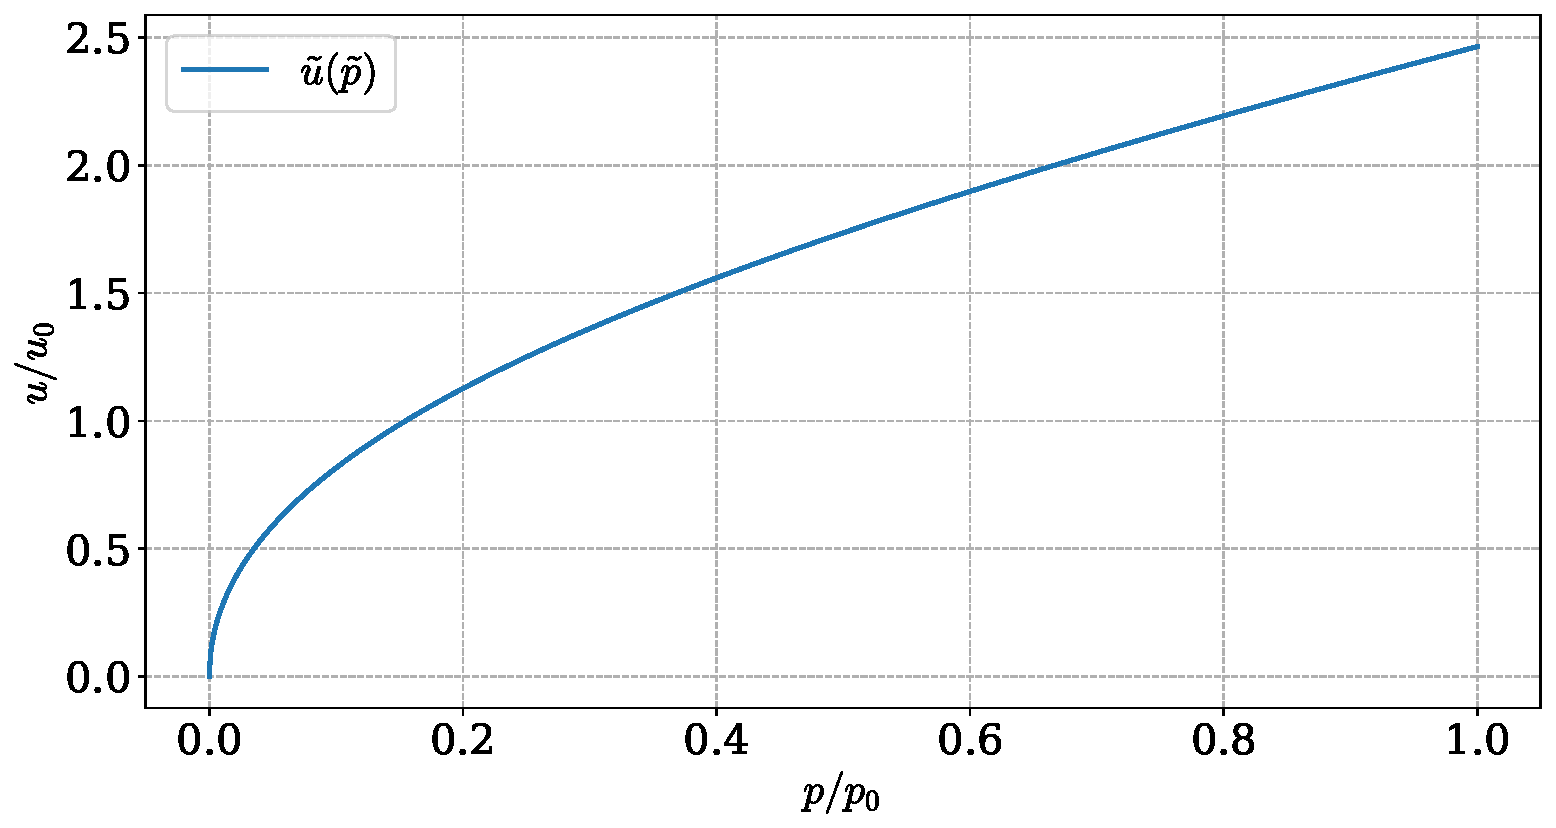
\includegraphics[width=0.6\textwidth]{../scripts/figurer/pion_tree_eos.pdf}
\end{figure}


\subsection{units}

The characteristic mass and length, as discussed in \autoref{section: TOV equation}, are found by setting $k_1 = k_2 = k_3 = 1$.
These are the dimensionless constants of the TOV equation, \autoref{dimensionless constants TOV}.
At tree-level, the bare constants $f$ and $\bar m$ are related to physical constants by $f = f_\pi$ and $m = m_\pi$, the pion decay constant and the pion mass.
Using the values for $f_\pi$ and $m_\pi$ as given in \autoref{section: units} and reinstating $c$ and $\hbar$, the values are
%
\begin{align}
    u_0 & =m_\pi^2 f_\pi^2 \frac{c}{\hbar^3}
    = 3.216\cdot 10^{33} \, \text{J}\,\text{m}^{-3}, \\
    m_0 & = \frac{c^4}{\sqrt{\frac{4 \pi}{ 3} u_0 G}} = 64.21\, M_\odot, \\
    r_0 & = \frac{G}{c^2} m_0 = 94.79 \, \text{km}.
\end{align}
%


\subsection{Results}

\begin{figure}[h]
    \centering
    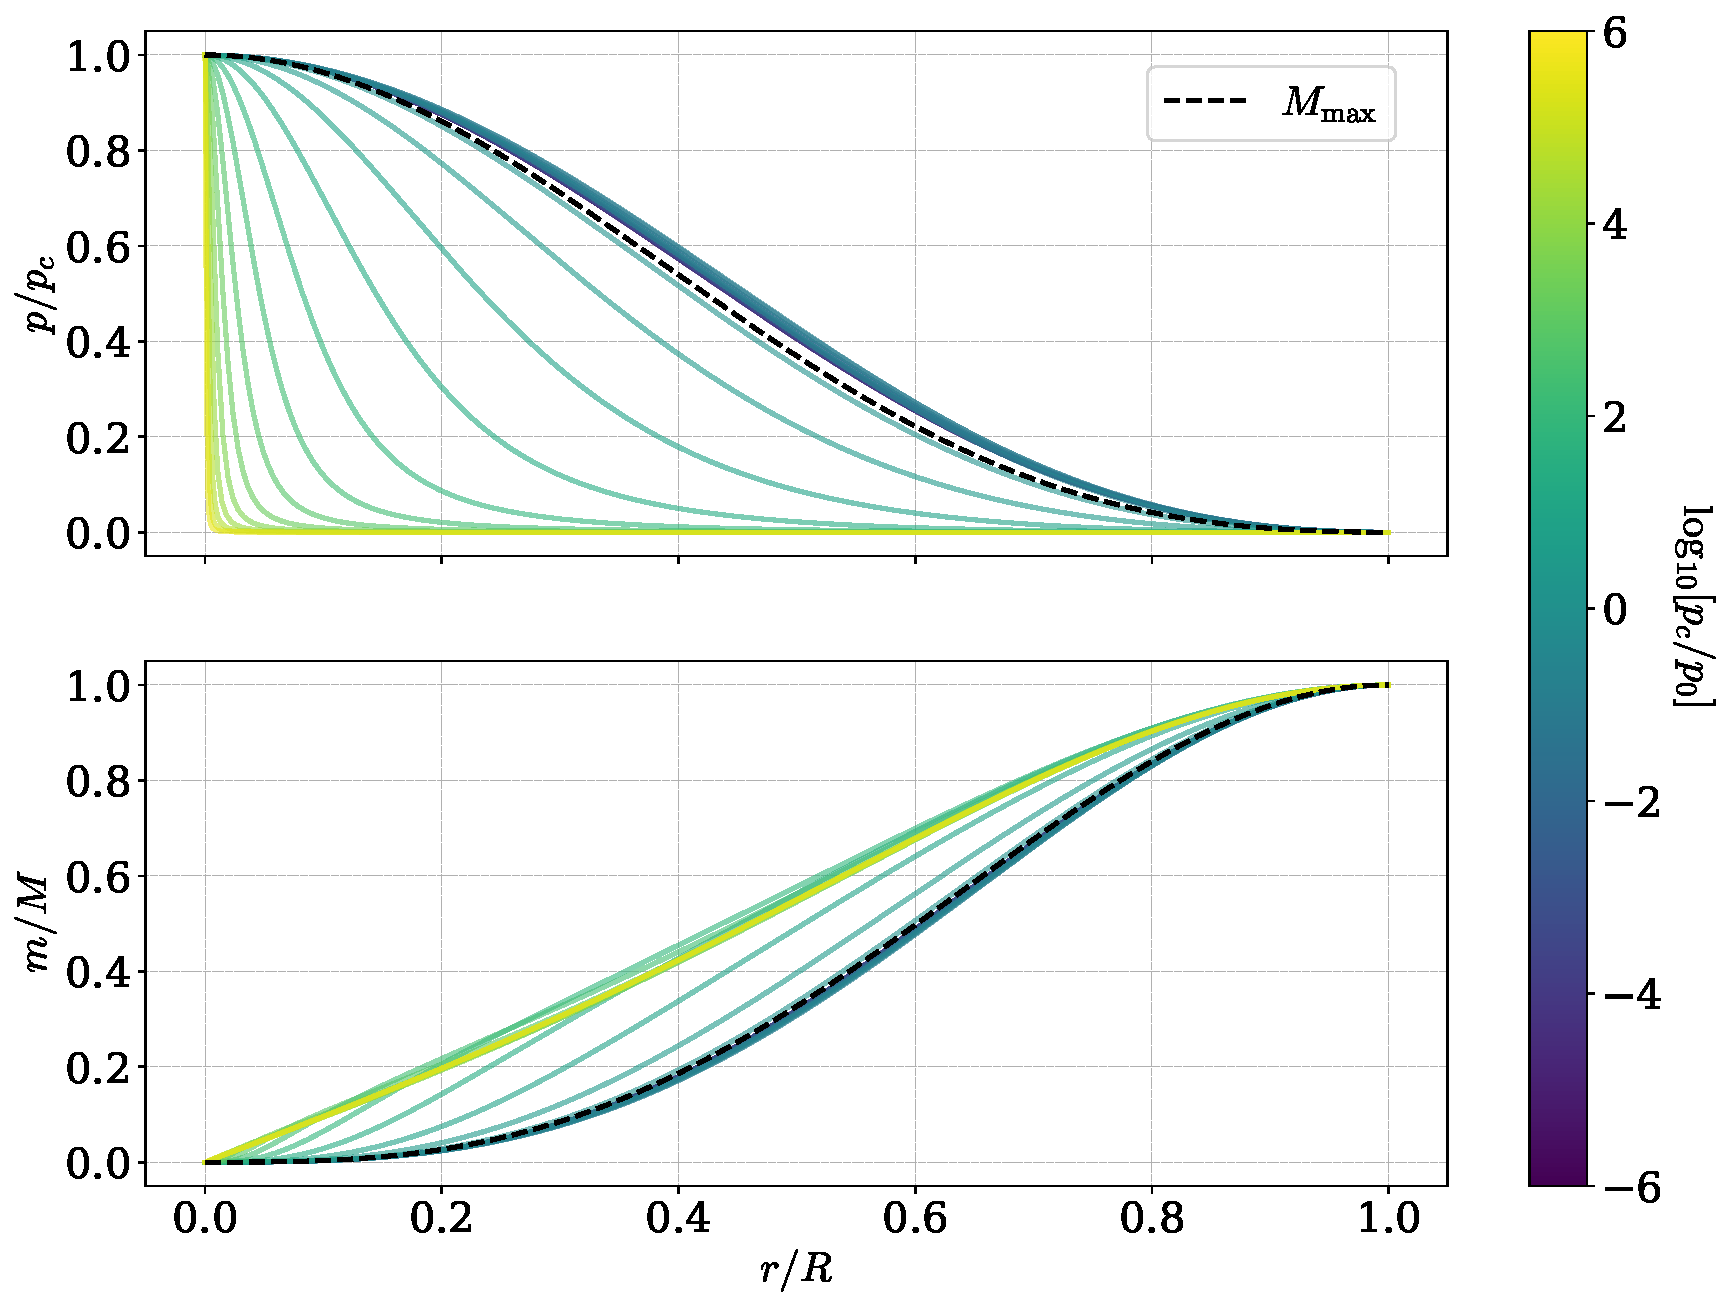
\includegraphics[width=0.8\textwidth]{../scripts/figurer/pressure_mass_pion_star.pdf}
\end{figure}


\begin{figure}[h]
    \centering
    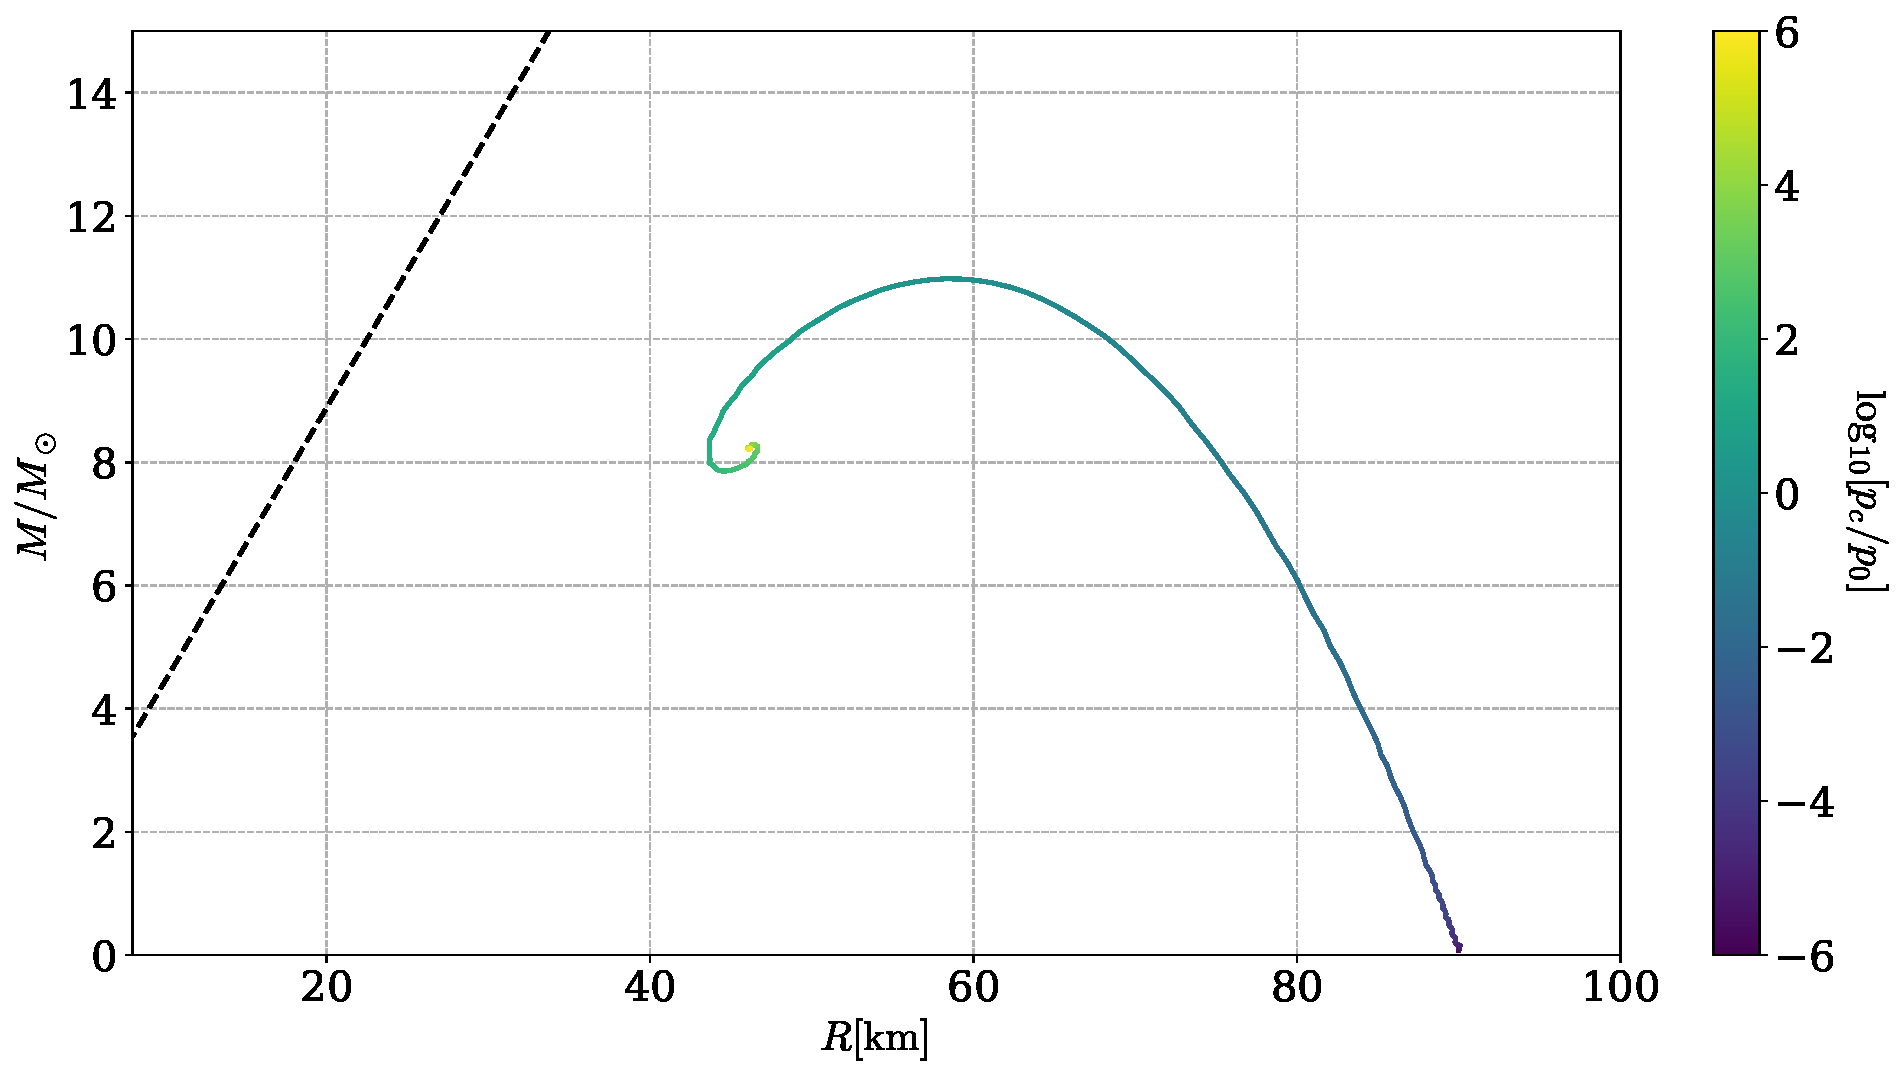
\includegraphics[width=0.95\textwidth]{../scripts/figurer/mass_radius_pion_star_tree.pdf}
\end{figure}

